%!TEX root = paper.tex
%%%%%%%%%%%%%%%%%%%%%%%%%%%%%%%%%%%%%%%%%%%%%%%%%%%%%%%%%%%%%%%%%%%%%%%%%%%%%%%
\section{User Perspective and Prospects}
\label{sec:engagement}

To get a grasp of the value of the introduced platforms, this section examines the users' perspective of gaming services, following a two-pronged approach. The first part introduces and discusses possible engagement metrics applicable to such services, while the second portion assembles some temporal cost-benefit models for hypothetical platform customers.


%%%%%%%%%%%%%%%%%%%%%%%%%%%%%%%%%%%%%%%%%%%%%%%%%%%%%%%%%%%%%%%%%%%%%%%%%%%%%%%%
\subsection{Engagement Metrics}

Metrics for user engagement, defined as ``\textit{the quality of the user experience that emphasises the positive aspects of the interaction, and in particular the phenomena associated with being captivated by a web application, and so being motivated to use it}''\cite{Lehmann2012}, can be used to compare different services against each other. The problem with engagement is finding the right measures befitting the type of service under scrutiny, in this case gaming, and cloud gaming in particular.

\begin{table*}
\centering
\caption{Overview of some simple engagement metrics comparing the three investigated services. Length data from \hltb, review scores from \metacritic.}
\label{tab:basic-engagement}
	\begin{tabu}{X[1.5]|X[r]X[r]X[r]X[r]X[r]X[r]X[r]X[r]X[r]}
	\toprule
	Service & Titles & Age Mean & Age $\sigma$ & Length Mean & Length $\sigma$ & Score Mean & Score $\sigma$ & User Score Mean & User Score $\sigma$\\
	\midrule
	\gfnow & $68$ & $2.38$ & $1.95$ & \SI{14.59}{\hour} & \SI{14.80}{\hour} & $76.12$ & $9.57$ & $72.55$ & $12.61$\\
	\psnow & $252$ & $4.27$ & $2.24$ & \SI{14.59}{\hour} & \SI{16.98}{\hour} & $73.33$ & $13.18$ & $70.77$ & $13.29$\\
	\steam & $7749$ & $2.86$ & $3.96$ & \SI{13.06}{\hour} & \SI{20.91}{\hour} & $71.00$ & $12.00$ & $69.04$ & $15.24$\\
	\bottomrule
	\end{tabu}
\end{table*}

So, what does engage gamers? Compared to video content and video streaming platforms this might be harder to answer due to the diversity of both games as well as gamers. Looking at some simple summary metrics in Tab.~\ref{tab:basic-engagement} does not give a very clear picture, with one exception: the number of titles. Being relatively young services, the two streaming platforms of note have a very limited total set of games available to them when compared to just the games available on \steam, which in itself again just represents a subset of all games available either solely on the PC (\metacritic lists $16192$) or across all platforms ($45803$ listed on the site). Due to the nature of the cloud services (streaming existing games) there are also no ``platform exclusive'' titles, which often increases the attractiveness of a specific platform for specific audiences. These limits on variety might be one reason why \steam is more compelling to wider audiences.

The age of video games might also be a deciding factor for a service. Besides some memorable classics, people should expect the most recent games to be available due to social factors and driven by advertisements and public appearances of the game. Looking at the high age of games this might not apply to cloud gaming platforms. The historic nature of \steam also increases its average game age, however coupled with a higher $\sigma$ representing the wider range of games also in their age. Additionally, \psnow might be a special case, as it is specifically advertised as a backwards compatibility for games that do not run on the latest Sony platform any more (the PlayStation 4 does not provide compatibility with its predecessors).






\begin{figure}[!t]
	\centering
	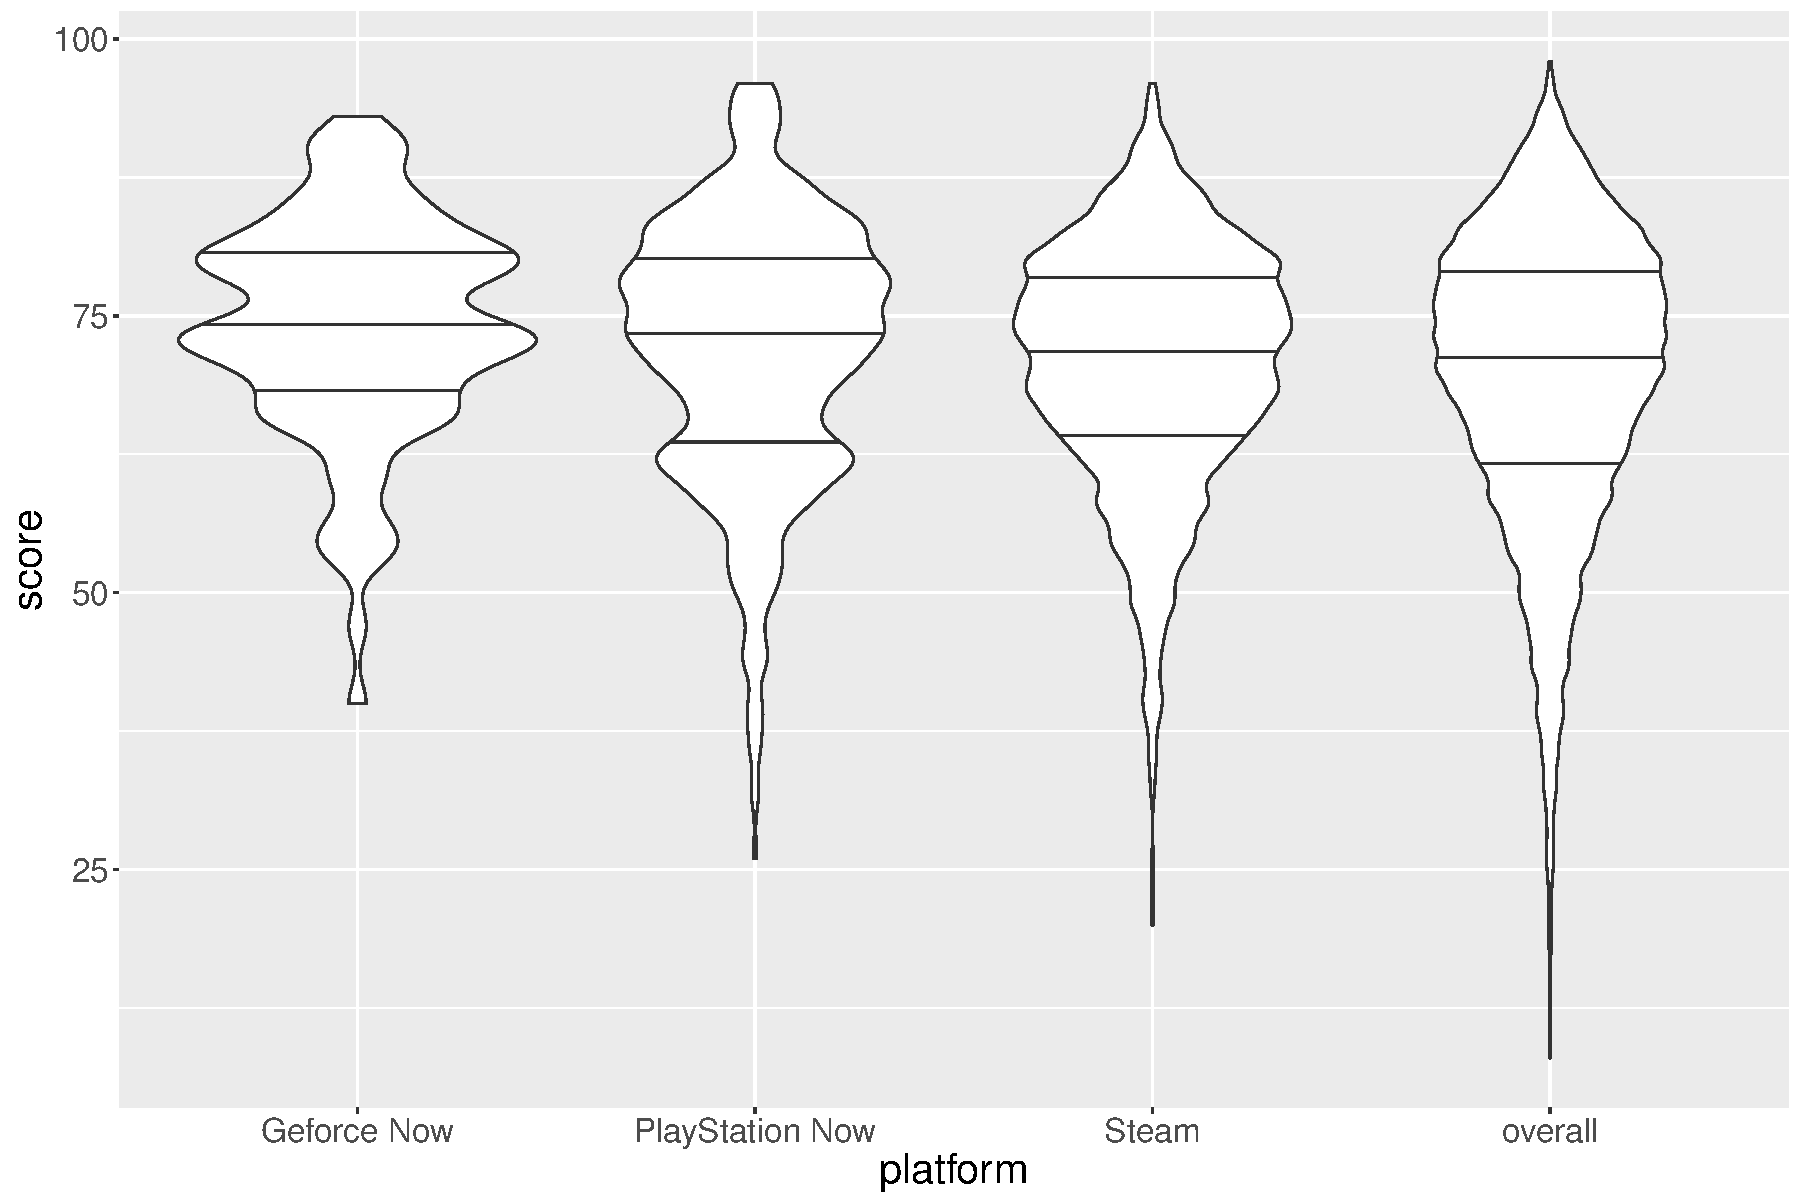
\includegraphics[width=1.0\columnwidth]{images/scores-by-platform-violin.pdf}
	\caption{Distribution of review scores across the investigated platforms, depicted as violin plot with $25\%$, $50\%$, $75\%$ quantiles drawn.}
\label{fig:scores-by-platform}
\end{figure}





%%%%%%%%%%%%%%%%%%%%%%%%%%%%%%%%%%%
\subsubsection{Validity of Metrics}

\todo[inline]{SV: Die Korrelationskoeffizienten muessen auf Basis des neuen Datensatzes neu berechnet werden.}

% Input by Svenja
After having had a closer look at the merged dataset, several possible relationships between metrics emerge. The success of a game in this case was associated with the ownership, so the more people own a game, the more successful it is.

First of all a few correlation coefficients:
\begin{itemize}
	\item Metacritic score + ownership: 0.2174691 --> This indicates a small effect.
	\item Metacritic user score + ownership: 0.1000701 --> This indicates a small effect, but somehow smaller than the correlation above.
	\item Game length (combined length) + ownership: 0.1767494 --> This indicates a small effect. 
	\item Price + ownership: -0.02796098 --> No effect visible.
\end{itemize}

When plotting the most obvious factors (MC score, length and price) the effects become visually graspable (see figures \ref{fig:rel-score-owners}, \ref{fig:rel-combinedlength-owners} and \ref{fig:rel-price-owners}).

\begin{figure}[!t]
	\centering
	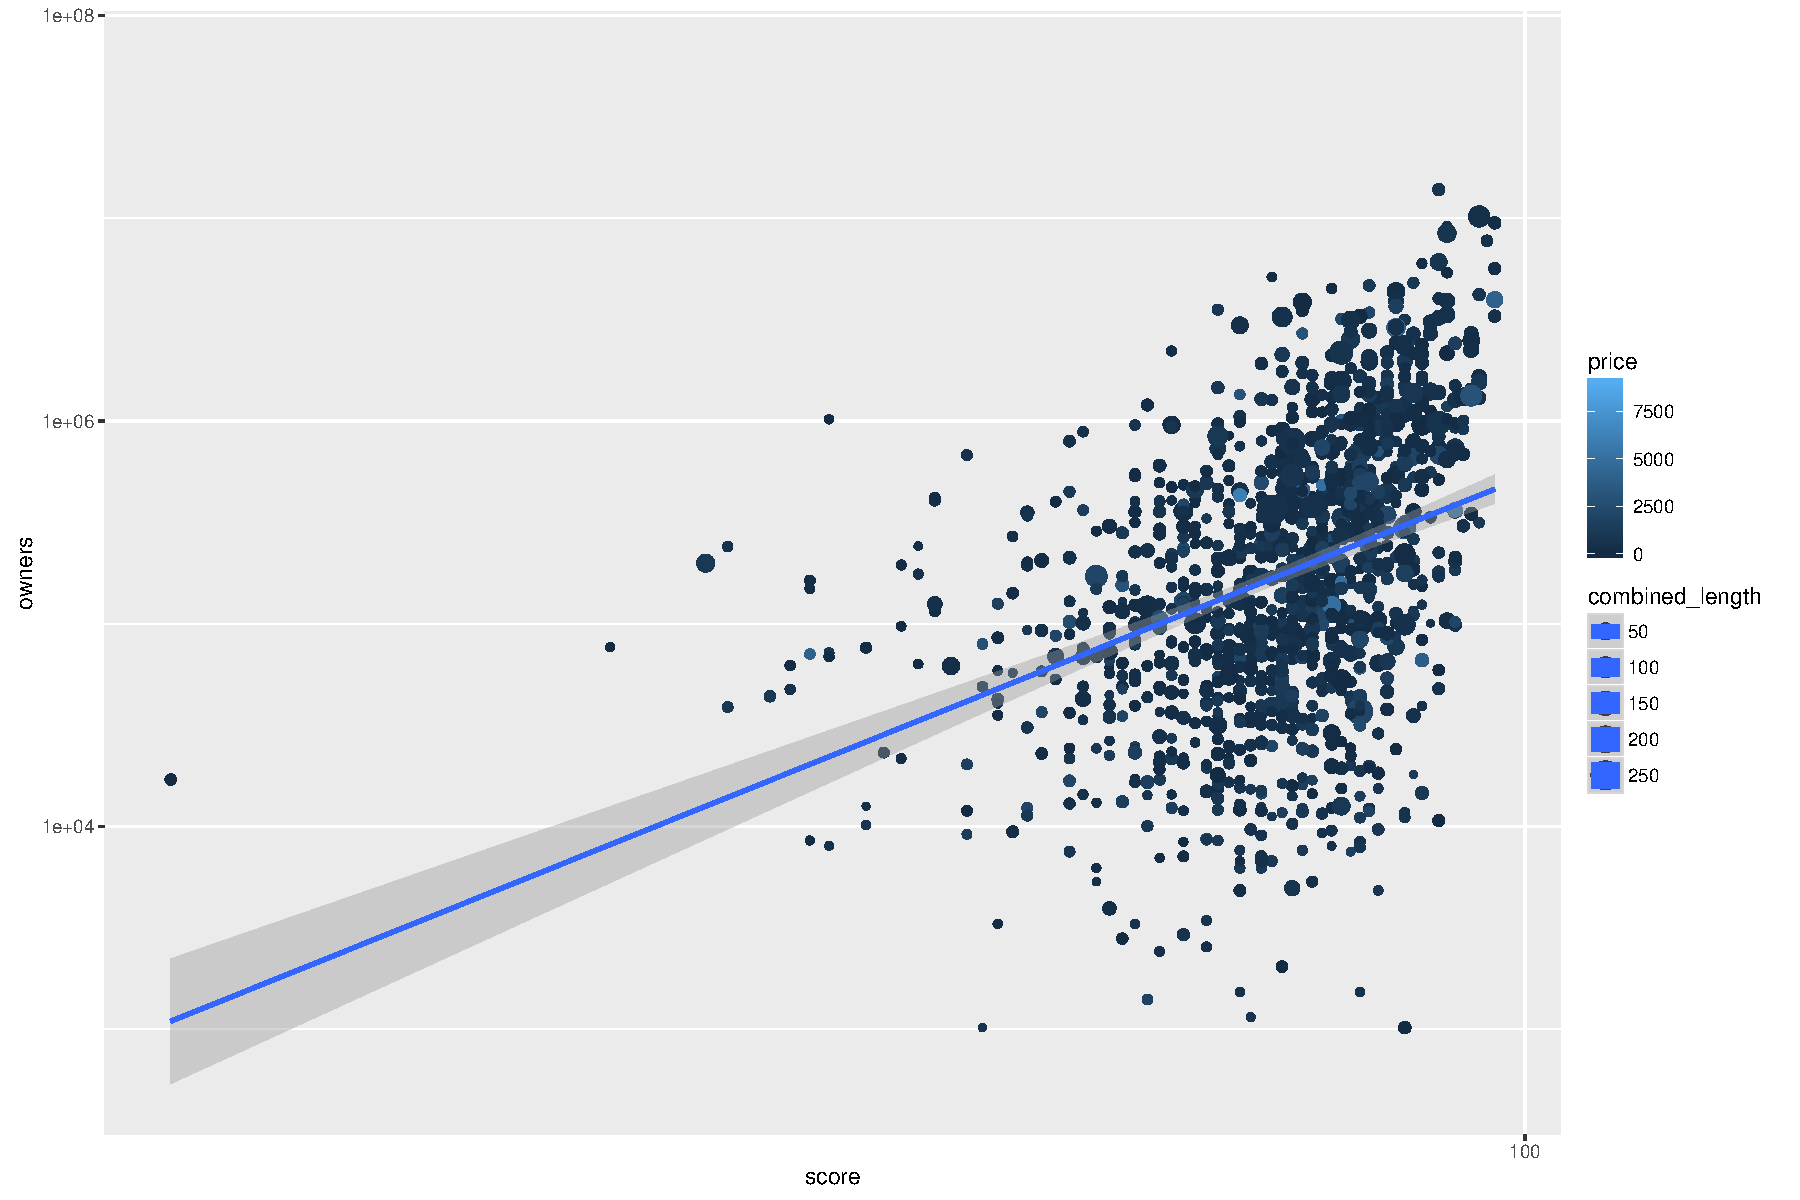
\includegraphics[width=1.0\columnwidth]{images/rel-score-owners.pdf}
	\caption{Relationship Metacritic score to ownership}
\label{fig:rel-score-owners}
\end{figure}

\begin{figure}[!t]
	\centering
	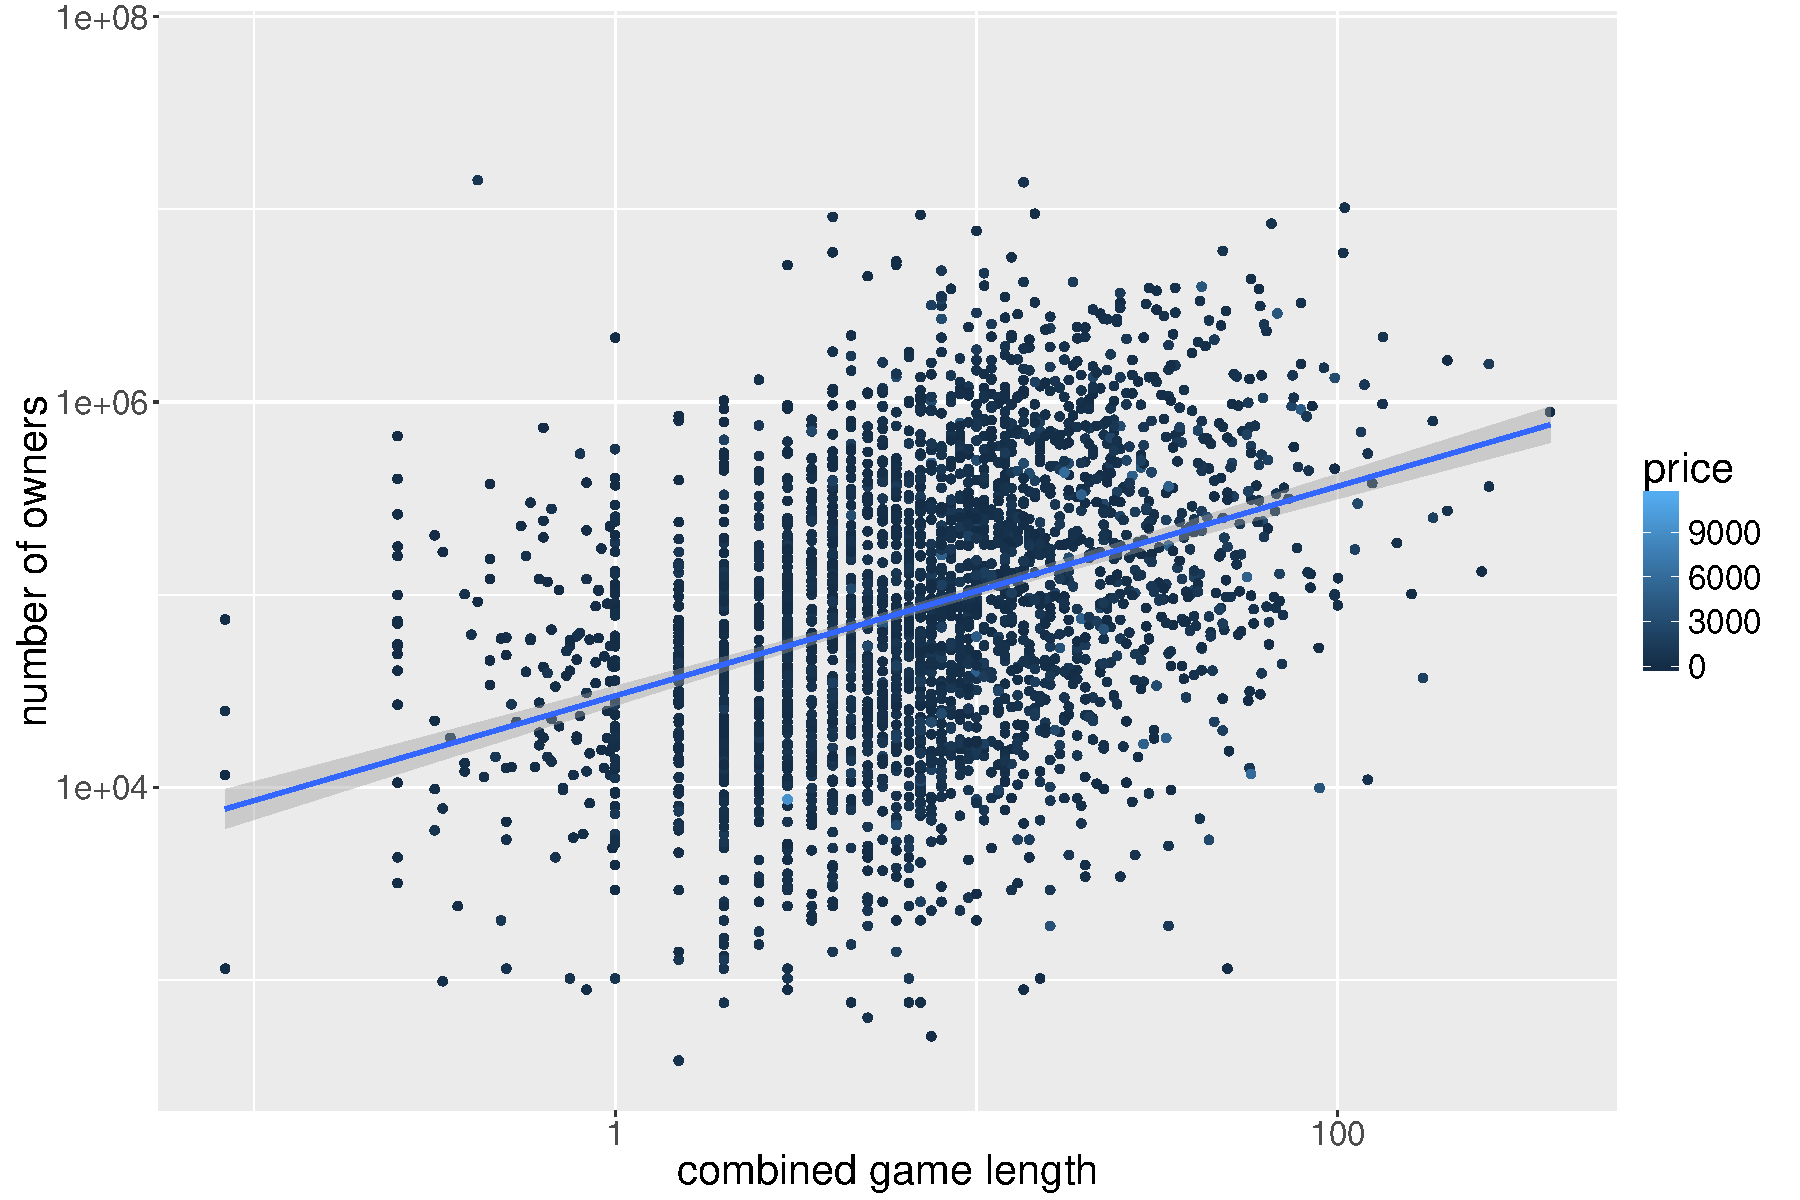
\includegraphics[width=1.0\columnwidth]{images/rel-combinedlength-owners.pdf}
	\caption{Relationship game length to ownership}
\label{fig:rel-combinedlength-owners}
\end{figure}

\begin{figure}[!t]
	\centering
	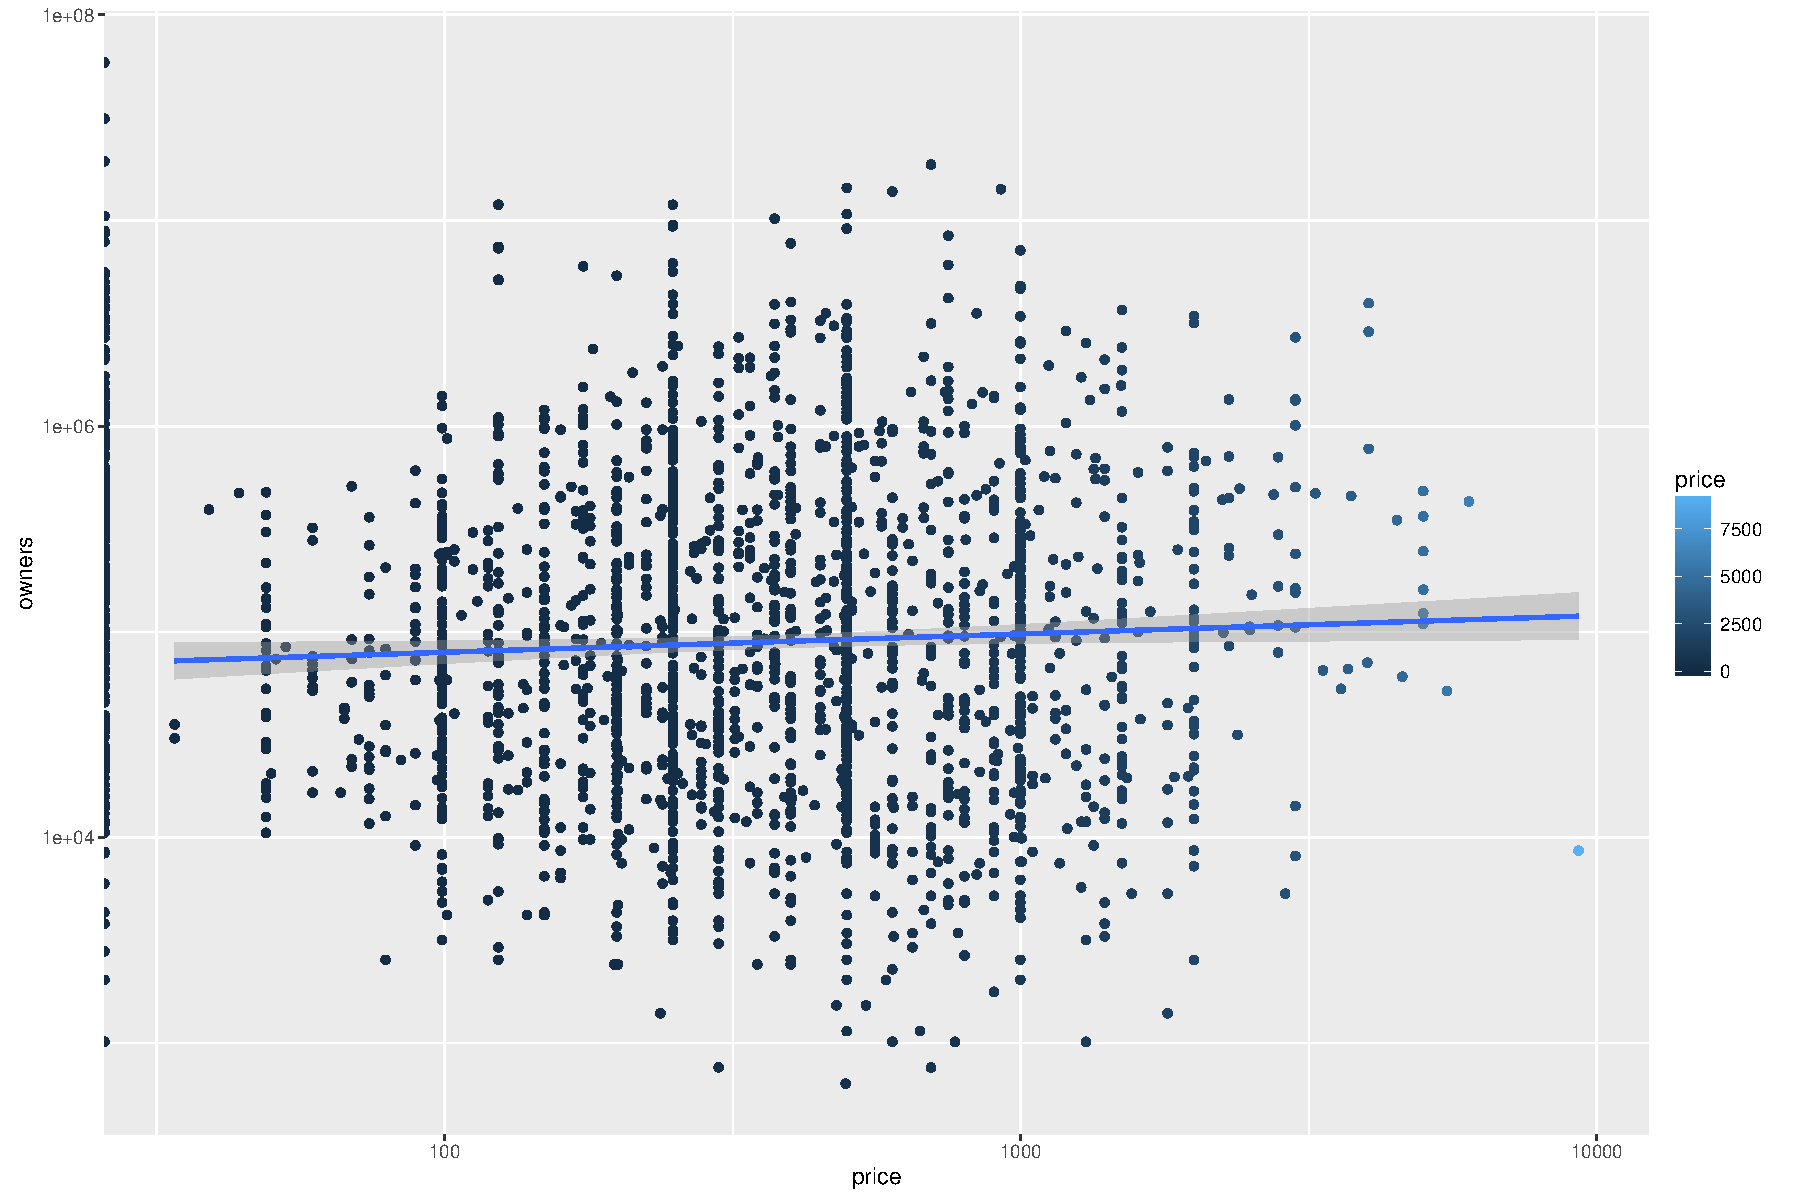
\includegraphics[width=1.0\columnwidth]{images/rel-price-owners.pdf}
	\caption{Relationship price to ownership}
\label{fig:rel-price-owners}
\end{figure}

However, when having a look at figures \ref{fig:rel-price-category-owners} and \ref{fig:rel-score-category-owners}, some details remain unclear: Despite having a relatively low Metacritic score, especially games within the 11-20 range seem to have quite a number of owners - why? Also, either games for free or expensive games seem to be popular. Maybe this is an indicator for the differentiation between hardcore and casual gamers? (Probably it would be interesting as well to track the price over the years and also weigh the ownership count relatively to a game's age.)

\begin{figure}[!t]
	\centering
	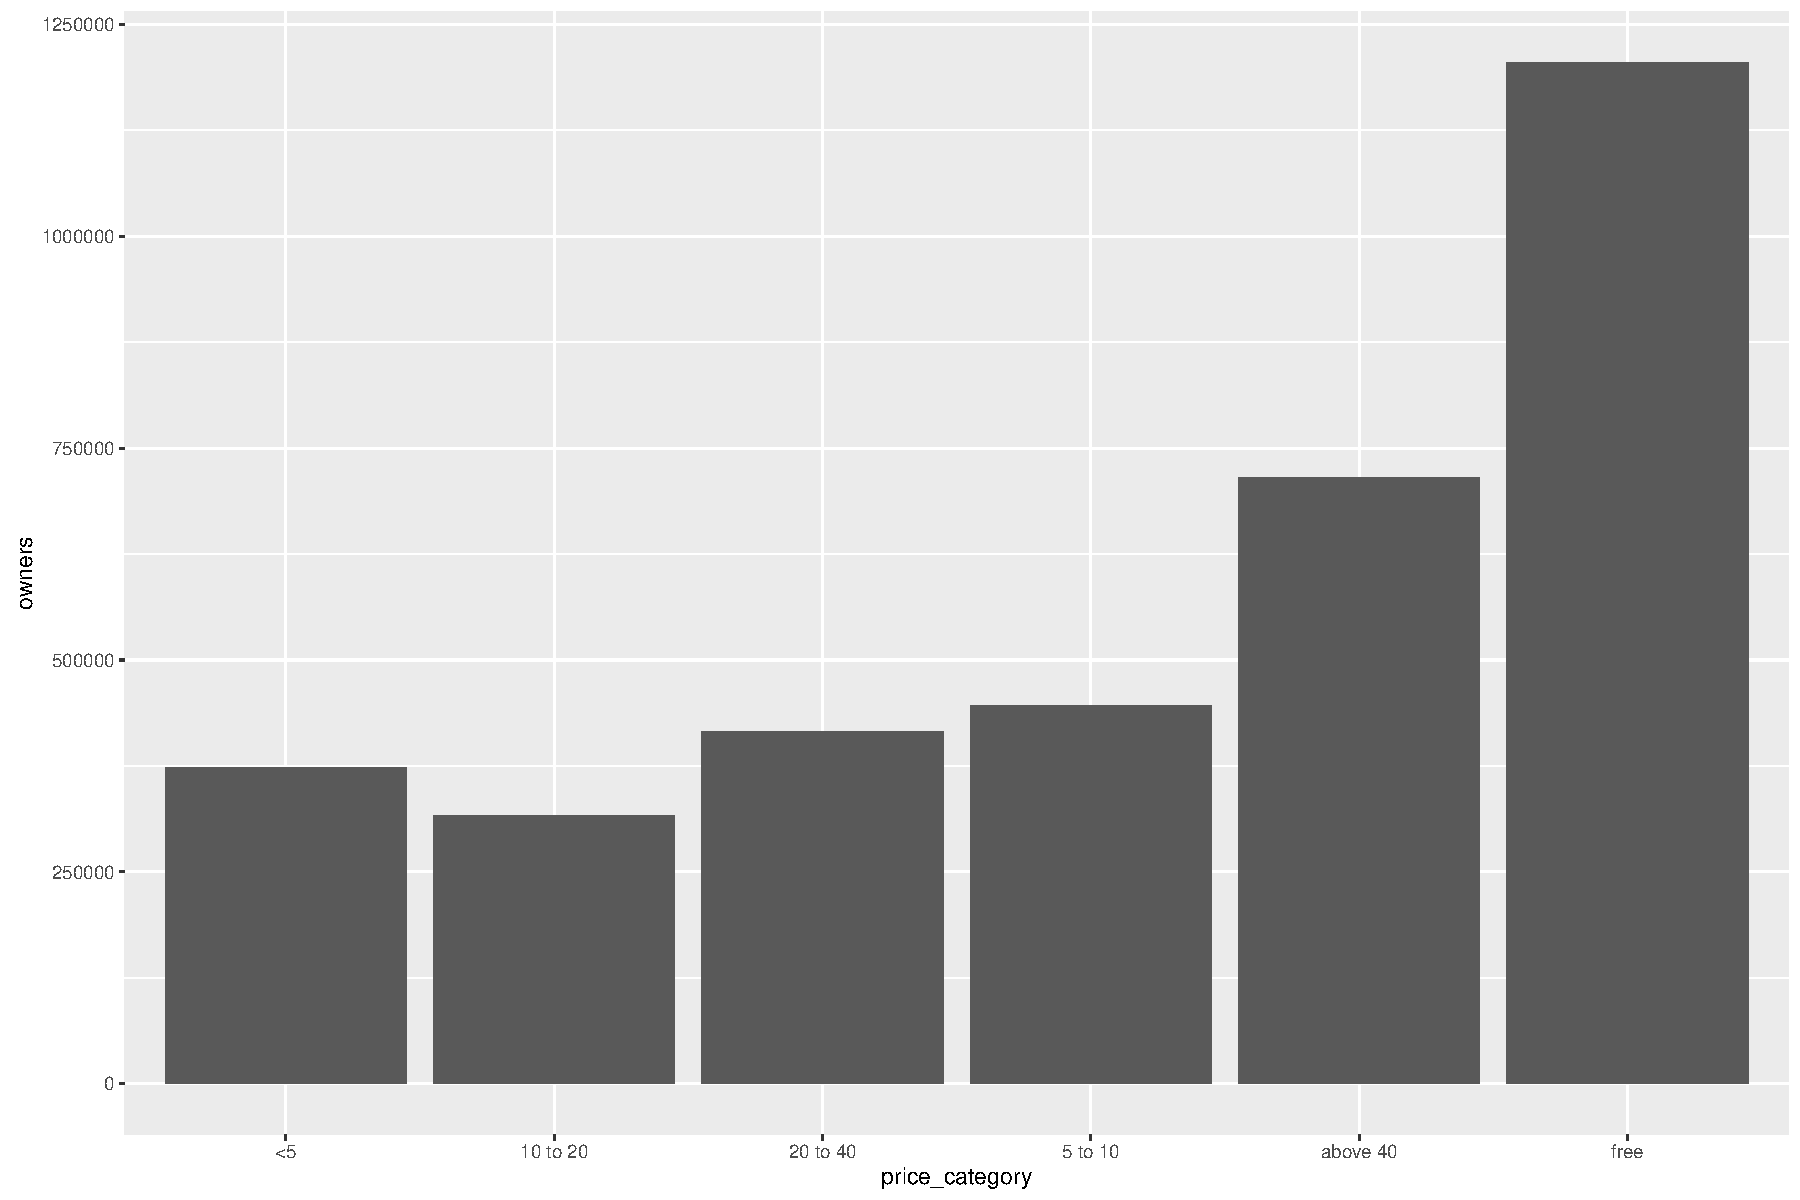
\includegraphics[width=1.0\columnwidth]{images/rel-price-category-owners.pdf}
	\caption{Relationship price category to ownership (\textbf{TODO: Bars need sorting})}
\label{fig:rel-price-category-owners}
\end{figure}

\begin{figure}[!t]
	\centering
	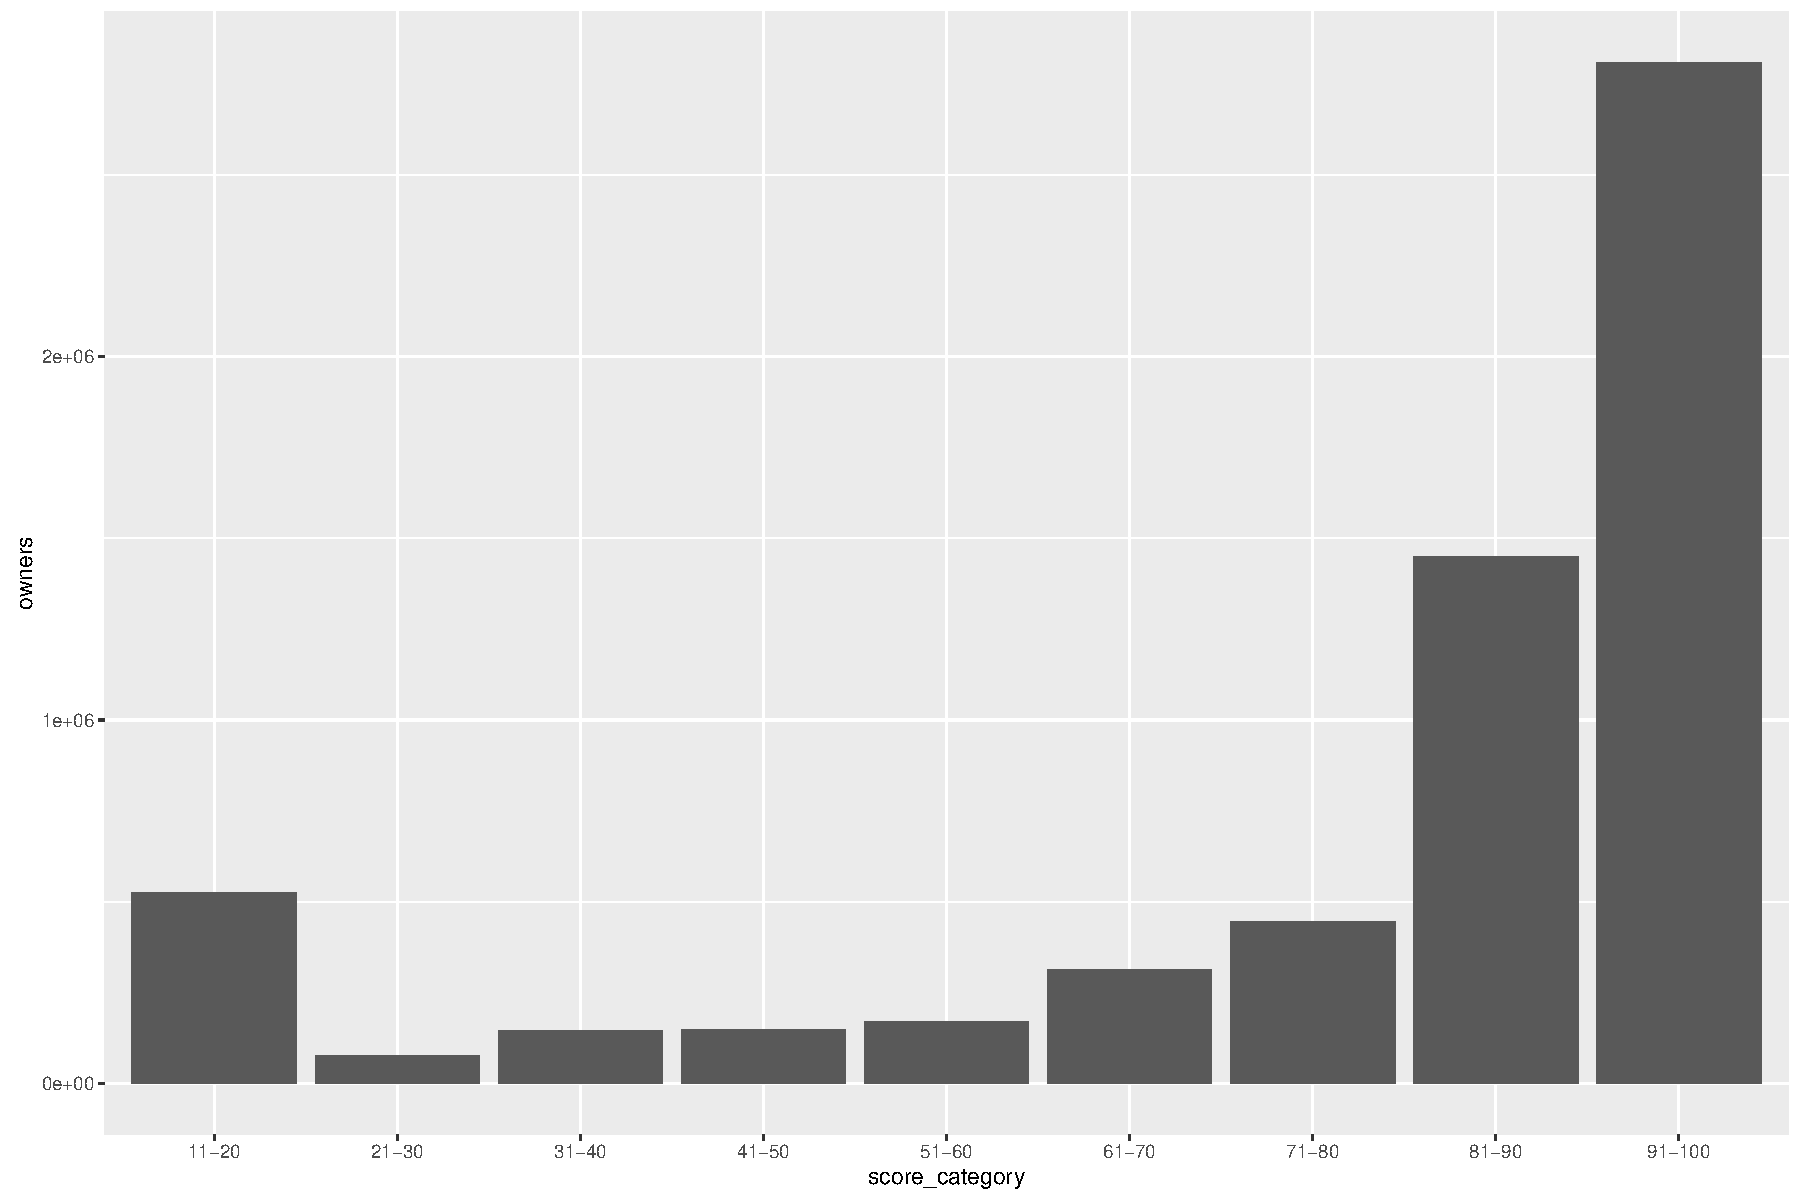
\includegraphics[width=1.0\columnwidth]{images/rel-score-category-owners.pdf}
	\caption{Relationship score category to ownership (\textbf{TODO: Bars need sorting})}
\label{fig:rel-score-category-owners}
\end{figure}

\subsubsection{Modelling Engagement Metrics}

\todo[inline]{SV: Ich probiers einfach mal ganz platt... Sollte natuerlich alles noch genormt sein. Man kann einzelne Spiele modellieren oder Systeme.}

\begin{equation}
\begin{split}
E_{game} = {newness} + {rating} +  {meanplaytime} \\+ {technicalprowess} - {specialhardwarecost} - {price}
\end{split}
\end{equation}

\begin{equation}
\begin{split}
E_{platform} = {newness} + {numberofgames} \\+ {technicalprowess} - {specialhardwarecosts}\\ - {runningcosts}
\end{split}
\end{equation}

%%%%%%%%%%%%
\subsubsection{Additional Factors}

\begin{itemize}
	\item Game costs and price history
	\item Number of platform ``exclusive'' titles?
	\item Other popularity measures? (e.g. steamspy owner data?)
	\item Variety and quality of game mechanics
	\item Required skill
	\item Story?
	\item Technical prowess, graphical fidelity, tightness/precision/quality of controls and game mechanics, e2e lag
	\item Hardware requirements of games?
\end{itemize}


%%%%%%%%%%%%%%%%%%%%%%%%%%%%%%%%%%%%%%%%%%%%%%%%%%%%%%%%%%%%%%%%%%%%%%%%%%%%%%%%
\subsection{Cost-Benefit Models}

Explicitly exempted in the previous engagement metrics was the factor price...



 hat den ersten Versuch einer Nutzenrechnung für Spieler auf verschiedenen Plattformen. Script könnte leicht angepasst und erweitert werden. Beispielausgabe \ref{fig:gamesperyear-over-budget}

\todo[inline]{PZ: Ist Grafik \ref{fig:games-over-years} die Basis fuer die Steigung bei ps now usw. ab dem Eintritt in Fig.~\ref{fig:gamesperyear-over-budget}. Ps now wuerde ich als Club Good sehen.}
\todo[inline]{FM: psnow/clubgood in the sense of a backwards compatibility service for devices that do not have native access to the streamed titles?.}


\begin{figure}[!t]
	\centering
	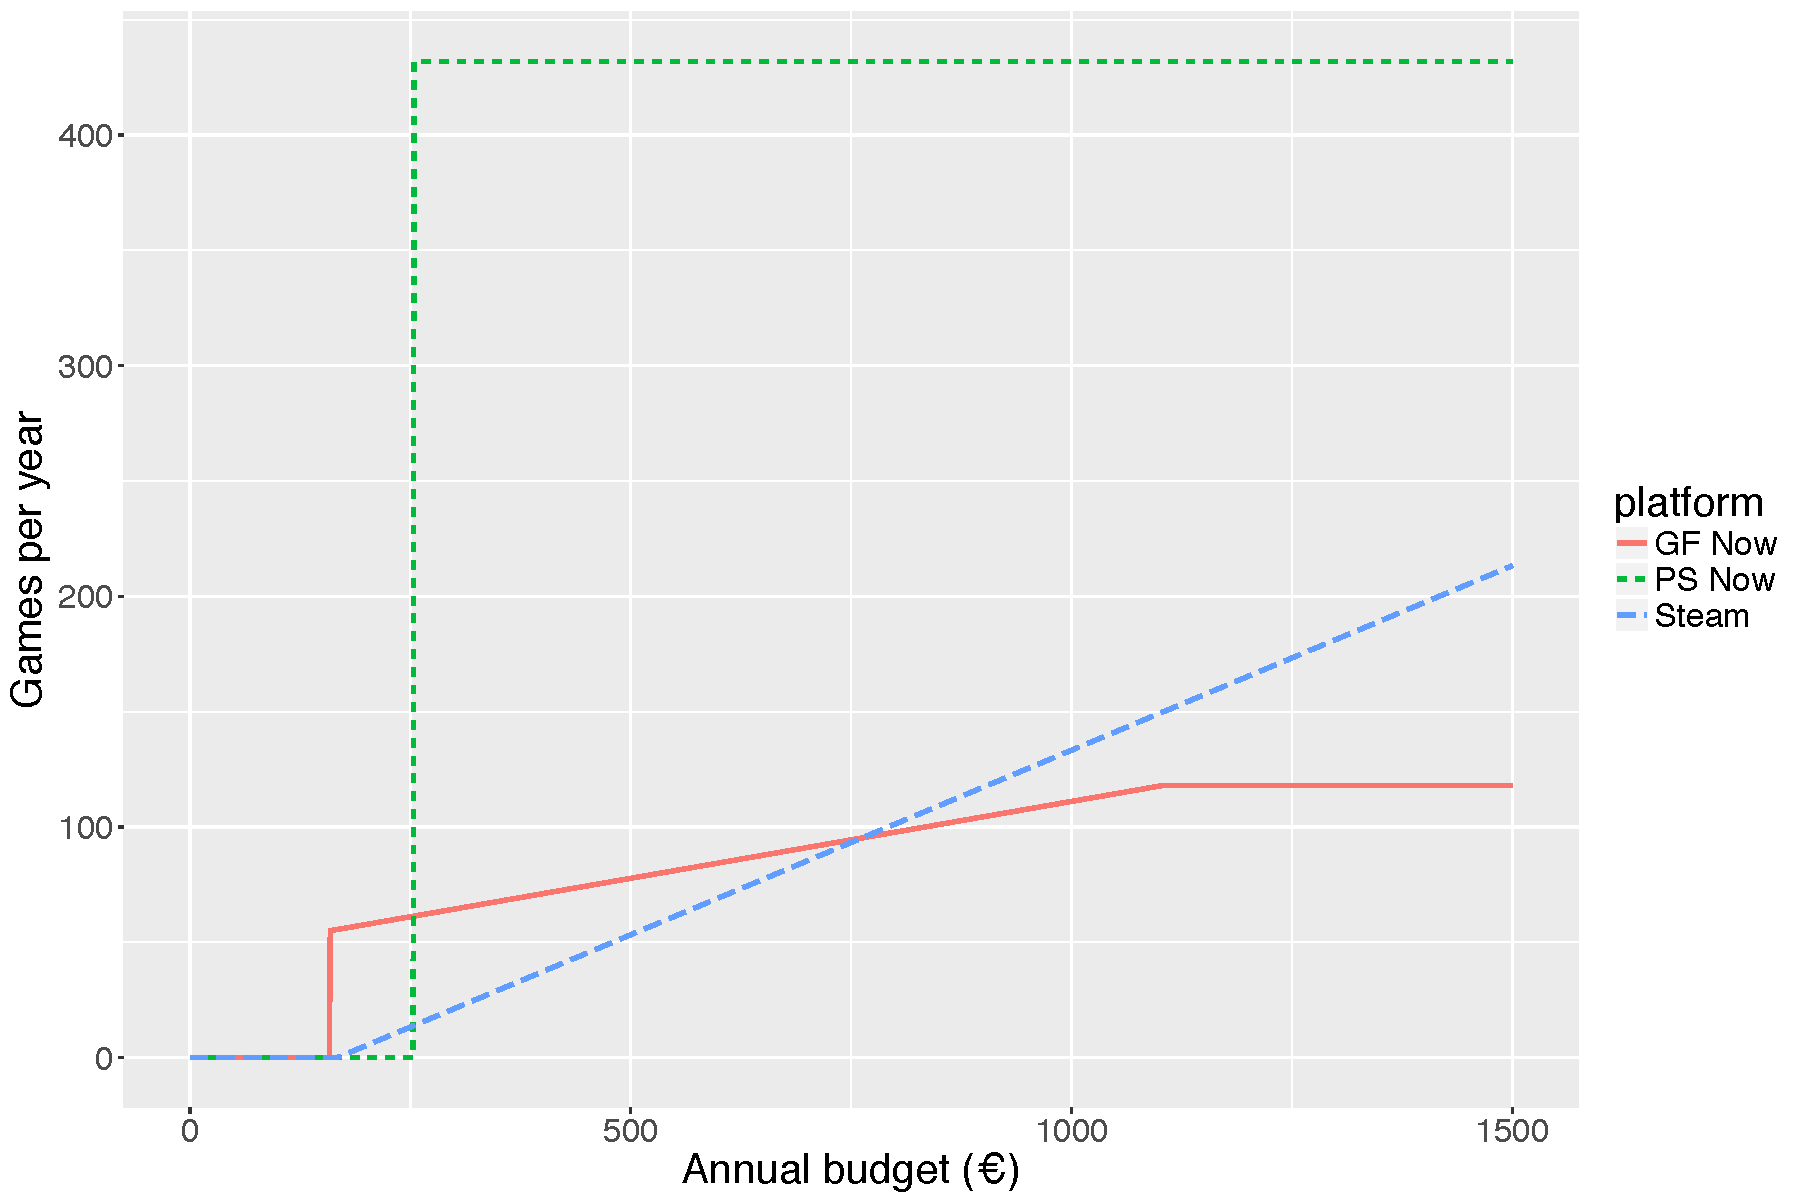
\includegraphics[width=1.0\columnwidth]{images/gamesperyear-over-budget.pdf}
	\caption{Models for several platforms showing the number of games per year that can be bought with a specific \$ budget.}
\label{fig:gamesperyear-over-budget}
\end{figure}

\begin{figure}[!t]
	\centering
	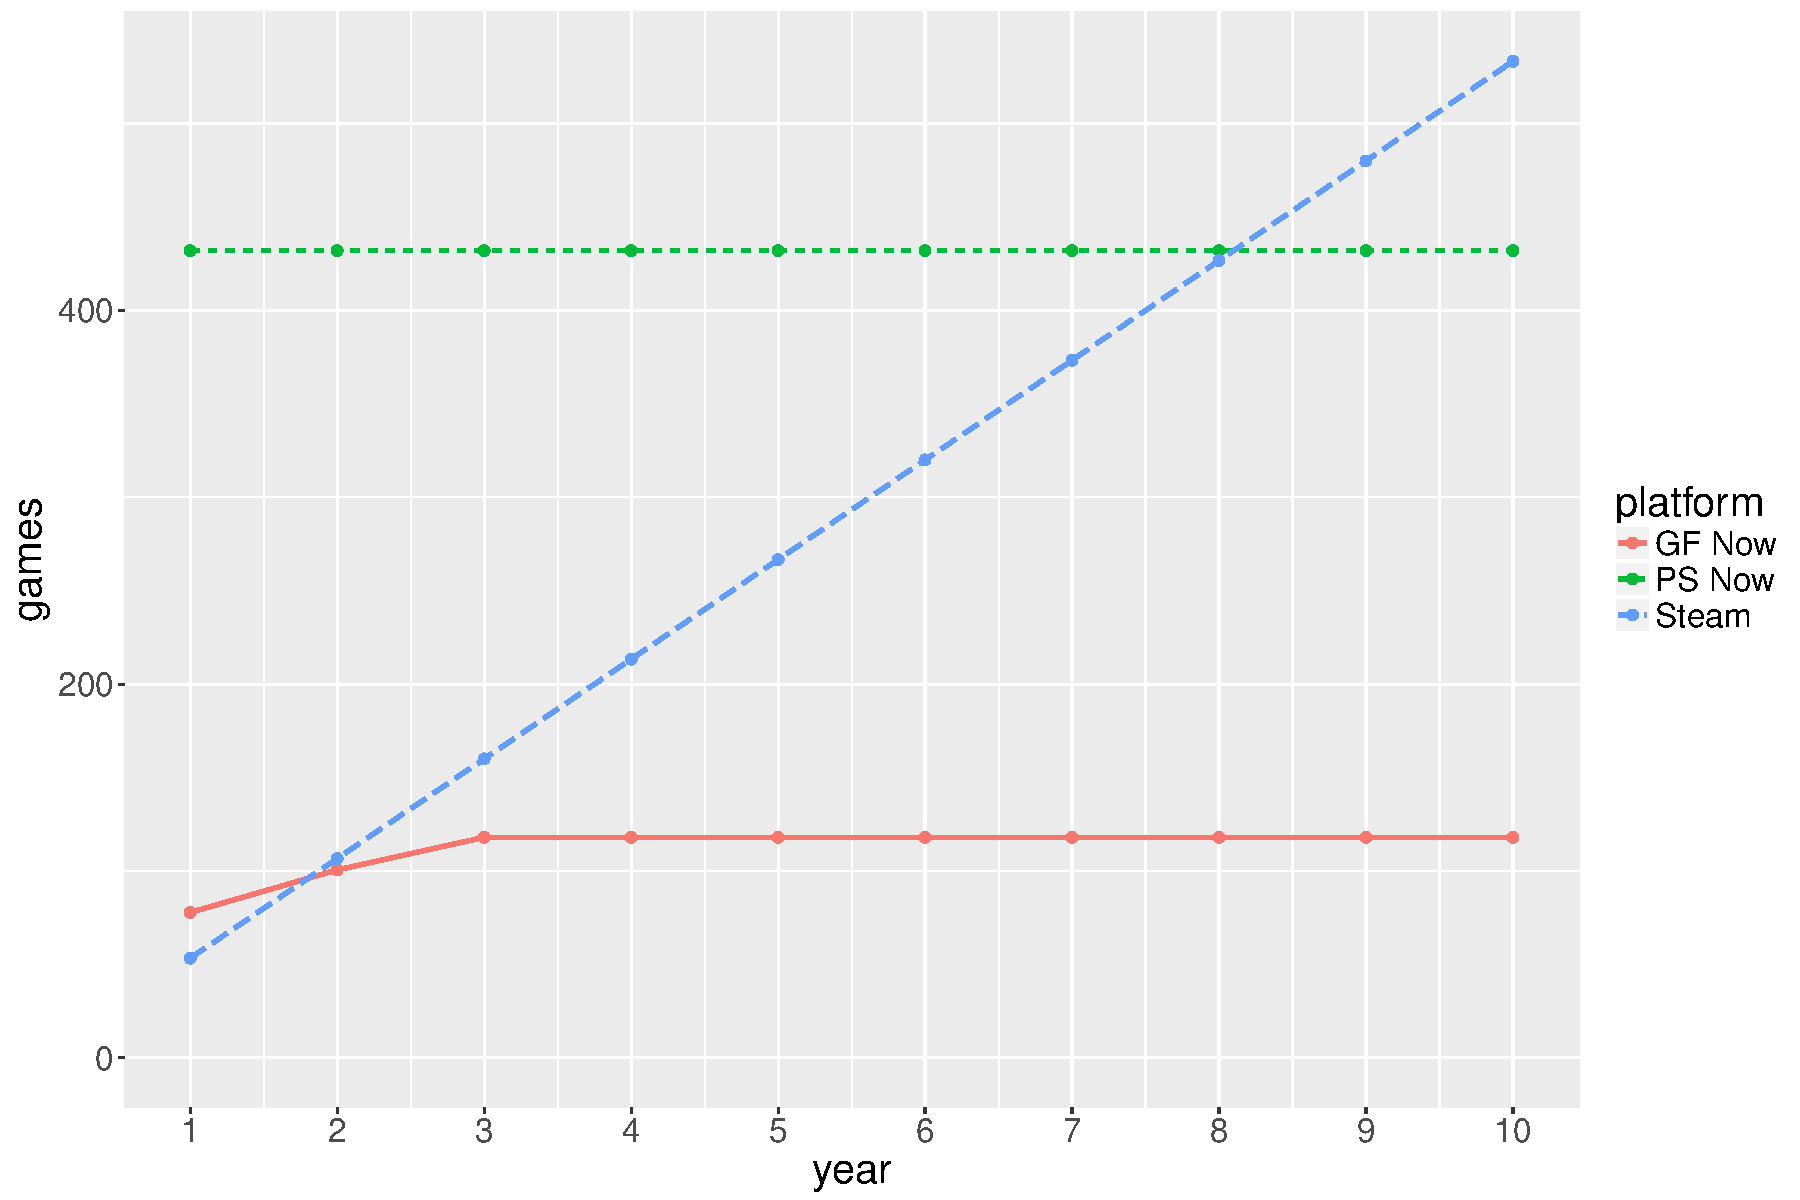
\includegraphics[width=1.0\columnwidth]{images/games-over-year.pdf}
	\caption{Models for several platforms showing the number of games that can be bought over the years subscribed to / using this service.}
\label{fig:games-over-years}
\end{figure}



%%%%%%%%%%%%%%%%%%%%%%%%%%%%%%%%%%%%%%%%%%%%%%%%%%%%%%%%%%%%%%%%%%%%%%%%%%%%%%%%
\subsection{Discussion}

PS Now specifically caters towards older titles and backwards compatability, may find a niche here
% wer ist die zielgruppe?
% was ist die beste platform?
% gibt es eine mainstream platform?
% unterschiedliche ausrichtungen?





% metacritic titles:
% PC 16192
% PS4 817
% XB1 588
% WiiU 474
% 3DS 871
% GFNOW 68
% PSNOW 243
% STEAM 7749



% \begin{figure}[!t]
% 	\centering
% 	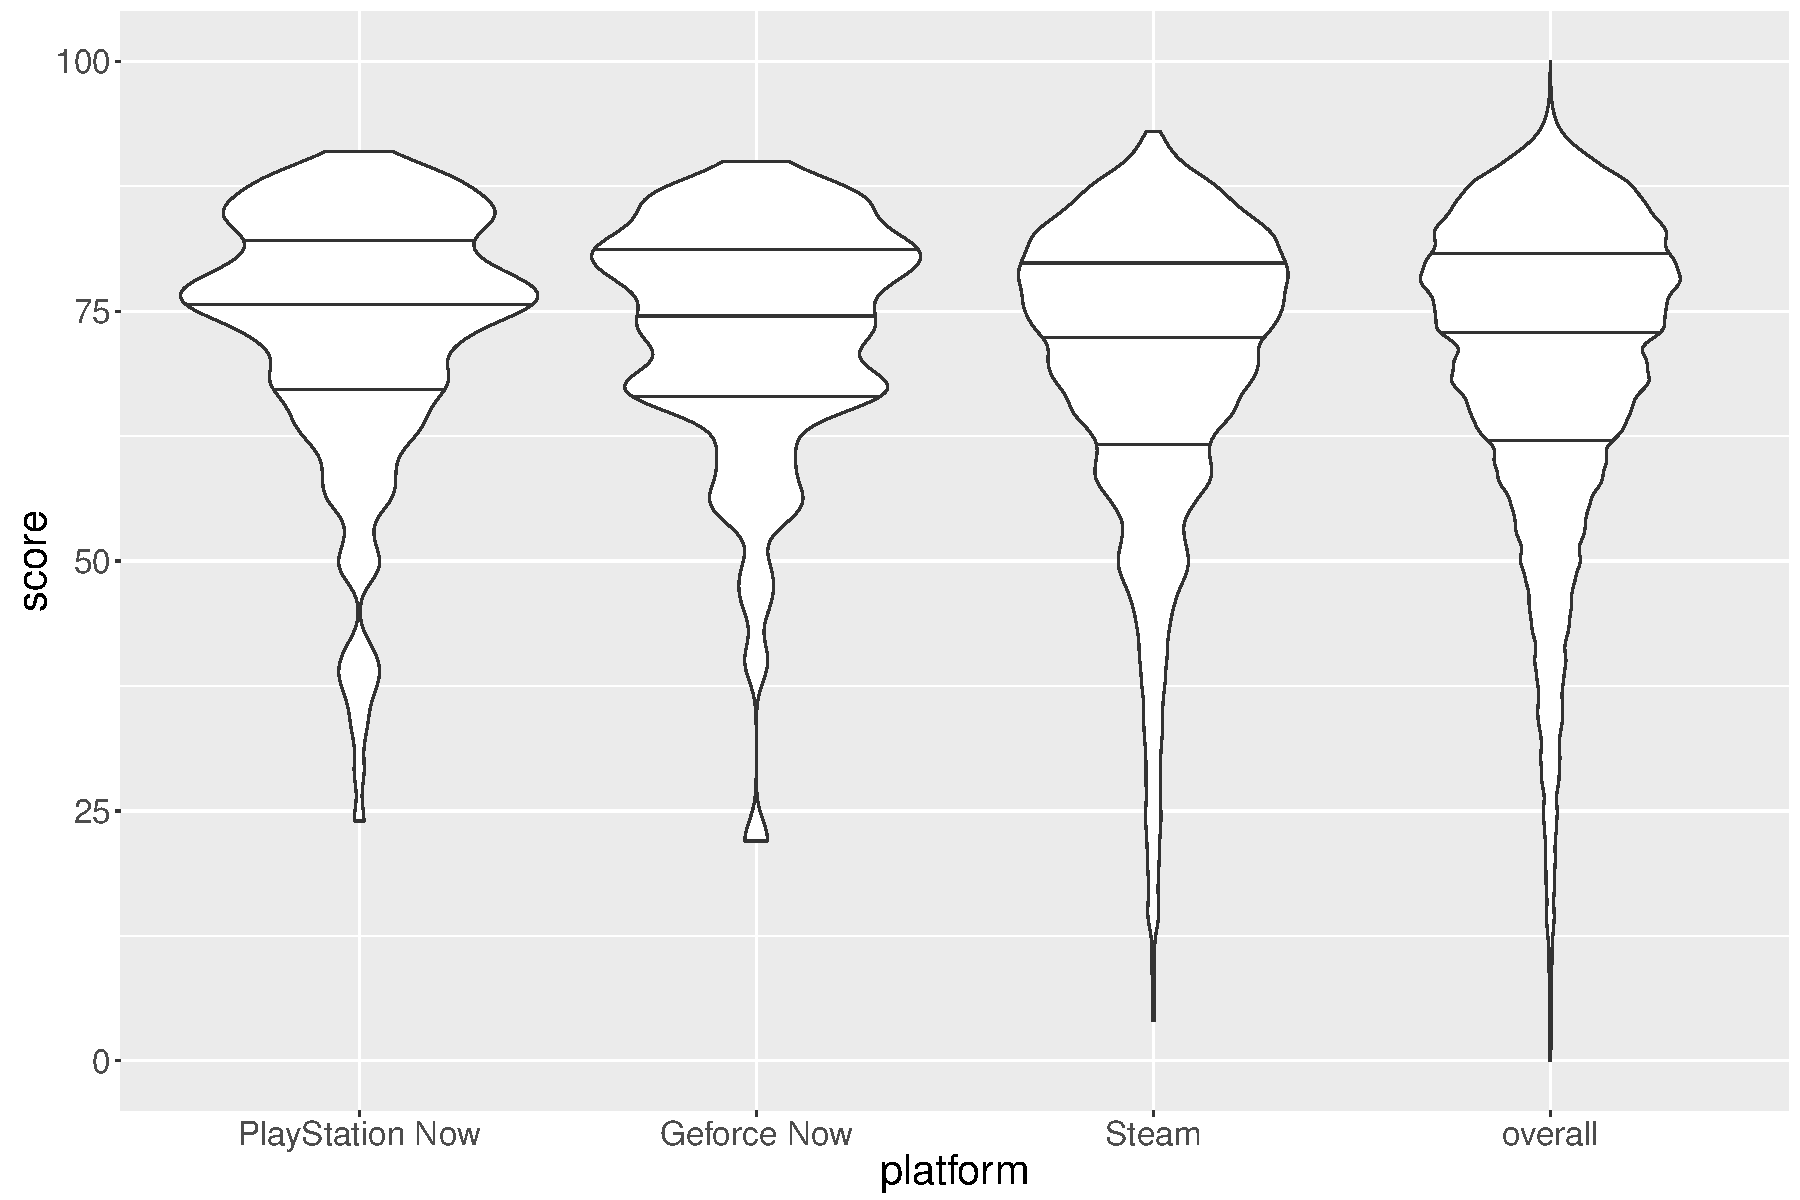
\includegraphics[width=1.0\columnwidth]{images/scores-by-platform-violin-userscore.pdf}
% 	\caption{Distribution of Metacritic user scores across the investigated platforms, depicted as violin plot with $25\%$, $50\%$, $75\%$ quantiles drawn.}
% \label{fig:userscores-by-platform}
% \end{figure}


% \subsection{E2E Lag}
% End-to-End Lag Model and Simulation in R. Now a standalone (submitted) paper at \url{https://github.com/mas-ude/onlinegame-lag-sim}. Can be referenced to argue the need for low E2E lag (meaning low network delay, but also the need for high fps).
